\documentclass{beamer}
\usepackage[slovene]{babel}
\usepackage[utf8]{inputenc}
\usepackage{lmodern}
\usepackage[T1]{fontenc}
\usetheme{Warsaw}
\usepackage{graphicx}
\mode<presentation>
\usepackage{latexsym}
\usepackage{amsmath}
\usepackage{amssymb}
\newtheorem{izrek}{Izrek}


\title[kratka predstavitev diplomskega dela]{Posplošena diskriminantna analiza z uporabo posplošenega singularnega razcepa } 
\author[Jernej Banevec]{Jernej Banevec\\
\medskip
{\small Mentor: izred. prof. dr. Marjeta Knez}
}
\institute[FMF] 
{
Fakulteta za matematiko in fiziko\\ 
\medskip
\textit{kratka predstavitev diplomskega dela} 
}
\date{8.11.2017} 

\begin{document}


\begin{frame}
\titlepage
\end{frame}

\begin{frame}
\frametitle{Pregled vsebine} 
\tableofcontents 
\end{frame}


\section{Posplošena diskriminantna analiza}

\begin{frame}
\frametitle{Posplošena diskriminantna analiza}
\begin{itemize}
\item Posplošitev linearne diskriminantne analize
\item Ena zelo uporabljenih statističnih metod
\item Oblike podatkov:
\begin{itemize}
\item Združeni v matriki $A \in \mathbb{R}^{mxn}$
\item m \ldots dimenzija posamezne meritve
\item n \ldots število meritev oz. podatkov
\item Podatki grupirani v k razredov oz. gruč
\end{itemize}
\end{itemize}
\end{frame}


\begin{frame}
\frametitle{Posplošena diskriminantna analiza}
\begin{itemize}
\item Iščemo preslikavo $$G : \mathbb{R}^m \rightarrow \mathbb{R}^\ell ,$$ kjer je $\ell \leqslant m - 1$
\item Cilj:
\begin{itemize}
\item Ohraniti razporejenost razredov
\item Zmanjšati razpršenost podatkov znotraj razredov
\item Povečati razlike med razredi
\end{itemize}
\end{itemize}
\end{frame}


\begin{frame}
\frametitle{Primerjava dobra proti slabi preslikavi}
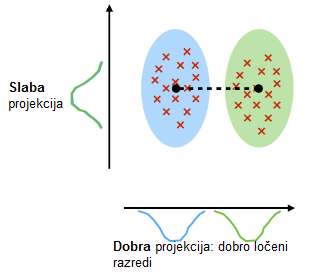
\includegraphics[scale = 0.85]{dobra-slaba}
\end{frame}


\begin{frame}
\frametitle{Definicije}
\begin{itemize}
\item Centroid i-tega razreda: $c^{(i)} = \frac{1}{n_i} \sum_{j \in N_i} a_j$
\item Centroid celotnih podatkov: $c = \frac{1}{n} \sum_{j = 1}^{n} a_j$
\item Matrika razpršenosti podatkov znotraj razreda: $$S_W = \sum_{i = 1}^{k} \sum_{j \in N_i}(a_j - c^{(i)})(a_j - c^{(i)})^T$$
\item Matrika razlik med razredi: $$S_B = \sum_{i = 1}^{k} n_i ( c^{(i)} - c)( c^{(i)} - c)^T$$
\item Matrika celotne razpršenosti: $$S_M = S_W + S_B$$
\item Tu so vse matrike elementi $\mathbb{R}^{mxm}$
\end{itemize}
\end{frame}


\begin{frame}
\frametitle{Definicije}
\begin{itemize}
\item Preslikava $S_W$ na prostor dimenzije $\ell$ : $$ S_{W}^{\ell} = G S_W G^T$$
\item Preslikava $S_B$ na prostor dimenzije $\ell$ : $$ S_{B}^{\ell} = G S_B G^T$$
\item Preslikava $S_M$ na prostor dimenzije $\ell$ : $$ S_{M}^{\ell} = G S_M G^T$$
\item Tu so vse matrike elementi $\mathbb{R}^{ \ell x \ell } $
\item $A^\ell = G A$
\end{itemize}
\end{frame}



\section{Posplošena diskriminantna analiza kot optimizacijski problem}

\begin{frame}
\frametitle{Posplošena diskriminantna analiza kot optimizacijski problem}
\begin{itemize}
%\item $ sled(S_W) = \sum_{i = 1}^{k} \sum_{j \in N_i}(a_j - c^{(i)})^T(a_j - c^{(i)}) = \sum_{i = 1}^{k} \sum_{j \in N_i} || a_j - c^{(i)}||_2^2$
%\item $ sled(S_B) = \sum_{i = 1}^{k}n_i( c^{(i)} - c)^T( c^{(i)} - c) = \sum_{i = 1}^{k} n_i || c^{(i)} - c||_2^2$
\item $ sled(S_W) = \sum_{i = 1}^{k} \sum_{j \in N_i} || a_j - c^{(i)}||_2^2$
\item $ sled(S_B) = \sum_{i = 1}^{k} n_i || c^{(i)} - c||_2^2$
\item Želimo:
\begin{itemize}
\item povečati $sled(S_B^\ell)$
\item zmanjšati $sled(S_W^\ell)$
\end{itemize}
\item Dobimo optimizacijski problem, pri katerem iščemo takšno preslikavo $G$, ki maksimizira
$$sled( G S_B G^T) / sled( G S_W G^T) \approx sled((S_W^\ell)^{-1}S_B^\ell)$$
\item Uporabno le ko je $S_W^\ell$ nesingularna oz. obrnljiva
\end{itemize}
\end{frame}


\section{Posplošen singularni razcep}

\begin{frame}
\frametitle{Posplošeni singularni razcep}
\begin{itemize}
\item Originalna definicija posplošenega singularnega razcepa (Van Loan)
\begin{izrek}[Posplošeni singularni razcep]
\label{izrek:GSVD} Za matriki $K_A \in \mathbb{R}^{pxm}$ z $p \geqslant m$ in $K_B \in \mathbb{R}^{nxm}$ obstajata ortogonalni matriki $U \in \mathbb{R}^{pxp}$ in $V \in \mathbb{R}^{nxn}$ ter nesingularna matrika $X \in \mathbb{R}^{mxm}$, da velja $$ U^T K_A X = diag(\alpha_1,..., \alpha_m) \ \text{in} \ V^T K_B X = diag(\beta_1,..., \beta_q) $$ kjer $q = min(n,m)$, $\alpha_i \geqslant 0$ za $1 \leqslant i \leqslant m$ in  $\beta_i \geqslant 0$ za  $1 \leqslant i \leqslant q$.
\end{izrek}
\item Pozneje dodatno posplošimo singularni razcep
\end{itemize}
\end{frame}


\section{Zgled}

\begin{frame}
\frametitle{Zgled - roža Iris}
\begin{itemize}
\item Precej poznan zgled
\item Trije razredi:
\begin{enumerate}
\item Iris - setosa
\item Iris - versicolor
\item Iris - virginica
\end{enumerate}
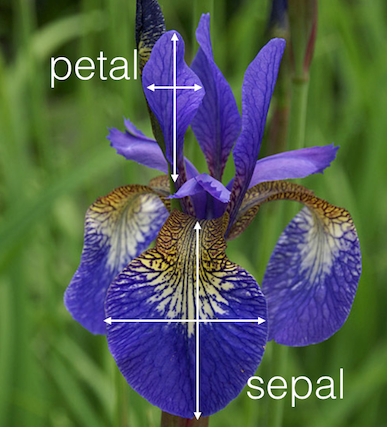
\includegraphics[scale = 0.30]{Iris1}
\end{itemize}
\end{frame}


\begin{frame}
\frametitle{Zgled - roža Iris}
\begin{itemize}
\item Podatki:
\[
A =
\begin{bmatrix}
	a_{1_{\text{sepal  length}}} & a_{2_{\text{sepal  length}}} & \cdots  & a_{150_{\text{sepal  length}}} \\
	a_{1_{\text{sepal  width}}} & a_{2_{\text{sepal width}}} & \cdots  & a_{150_{\text{sepal  width}}} \\
	a_{1_{\text{petal  length}}} & a_{2_{\text{petal  length}}} & \cdots  & a_{150_{\text{petal  length}}} \\
	a_{1_{\text{petal  width}}} & a_{2_{\text{petal  width}}} & \cdots  & a_{150_{\text{petal  width}}}
\end{bmatrix}
, Y = 
\begin{bmatrix}
	\omega_{\text{sitosa}}\\
	\omega_{\text{sitosa}}\\
	\vdots \\
	\omega_{\text{versicolor}}\\
	\vdots \\
	\omega_{\text{virginica}}
\end{bmatrix}
\]

\item Na teh podatkih uporabimo posplošeno diskriminantno analizo
\begin{enumerate}
\item Računanje centroidov
\item Računanje matrik razpršenosti podatkov
\item Lastni razcep $(S_W^\ell)^{-1}S_B^ \ell $
\item Urejanje lastnih vrednosti (po parih z vektorji)
\item Transformiranje na nov podprostor
\end{enumerate}
\end{itemize}
\end{frame}


\begin{frame}
\frametitle{Zgled - roža Iris}
\begin{itemize}
\item Slikamo na 2-dimenzionalen (pod)prostor
\item Dobimo sledečo sliko:
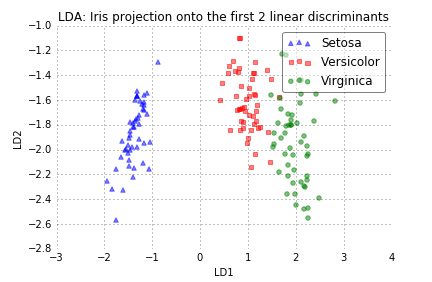
\includegraphics[scale = 0.65]{Iris3}
\end{itemize}
\end{frame}


\section{Viri}

\begin{frame}
\frametitle{Viri}
\begin{itemize}
\item Howland P. in Park H., Generalizing discriminant analysis using the generalizen singular value decomposition. TPAMI. 2004, 26, 8, 995-1006
\item Jieping Ye, Characterization of a Family of Algorithms for Generalized Discriminant Analysis on Undersampled Problems. Journal of Machine Learning Research. 2005, 6, 483–502
\end{itemize}
\end{frame}

\end{document}
